\begin{figure}[t]
\centering
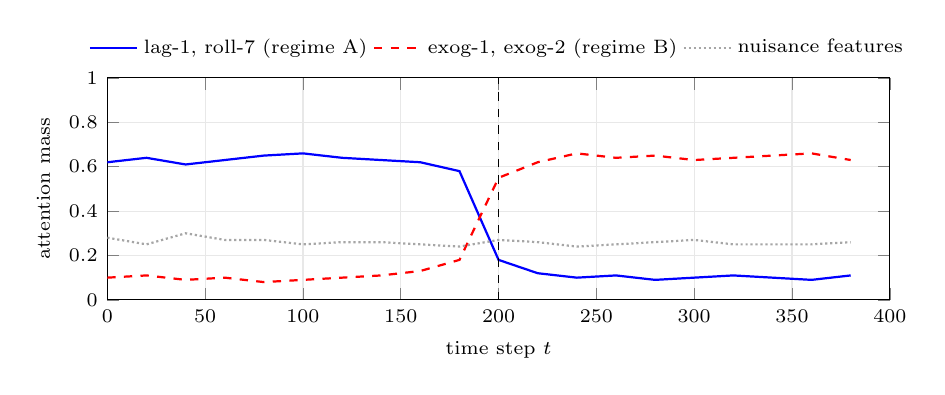
\begin{tikzpicture}
\begin{axis}[
    width=0.95\columnwidth,
    height=4.4cm,
    xlabel={time step $t$},
    ylabel={attention mass},
    ymin=0, ymax=1.0,
    xmin=0, xmax=400,
    legend style={font=\scriptsize, at={(0.5,1.04)}, anchor=south, legend columns=3, draw=none},
    tick label style={font=\scriptsize},
    label style={font=\scriptsize},
    grid=both,
    grid style={gray!18},
]
% regime A active features (lag1, roll7)
\addplot[blue, thick] coordinates {
(0,0.62)(20,0.64)(40,0.61)(60,0.63)(80,0.65)(100,0.66)(120,0.64)(140,0.63)(160,0.62)(180,0.58)
(200,0.18)(220,0.12)(240,0.10)(260,0.11)(280,0.09)(300,0.10)(320,0.11)(340,0.10)(360,0.09)(380,0.11)
};
\addlegendentry{lag-1, roll-7 (regime A)}
\addplot[red, thick, dashed] coordinates {
(0,0.10)(20,0.11)(40,0.09)(60,0.10)(80,0.08)(100,0.09)(120,0.10)(140,0.11)(160,0.13)(180,0.18)
(200,0.55)(220,0.62)(240,0.66)(260,0.64)(280,0.65)(300,0.63)(320,0.64)(340,0.65)(360,0.66)(380,0.63)
};
\addlegendentry{exog-1, exog-2 (regime B)}
\addplot[gray!70, thick, densely dotted] coordinates {
(0,0.28)(20,0.25)(40,0.30)(60,0.27)(80,0.27)(100,0.25)(120,0.26)(140,0.26)(160,0.25)(180,0.24)
(200,0.27)(220,0.26)(240,0.24)(260,0.25)(280,0.26)(300,0.27)(320,0.25)(340,0.25)(360,0.25)(380,0.26)
};
\addlegendentry{nuisance features}
\addplot[black, dashed] coordinates {(200,0) (200,1.0)};
\end{axis}
\end{tikzpicture}
\caption{Mean attention mass assigned by TAFS to three feature groups on the synthetic regime-switch task. The regime change at $t{=}200$ moves the informative subset from $\{\text{lag-1},\text{roll-7}\}$ (regime A) to $\{\text{exog-1},\text{exog-2}\}$ (regime B); TAFS re-allocates its attention within a small number of steps, while nuisance features remain suppressed.}
\label{fig:synth_regime}
\end{figure}
